\chapter{Compressors}

\section{Piston compressors}

\subsection{Introduction}

\subsection{Flow rate}

Figure \ref{pistoncomp_pvTS} displays the $p-V$ diagram and the $T-s$ diagram of a piston compressor's the ideal working cycle. The parts of the working cycle are: 1-2. intake (isobar), 2-3. isentropic compression, 3-4. isobar outlet, 4-1. isentropic expansion. 

The full volume of the piston ($V_{piston}$) consists of two parts: the stoke volume $V_{st}$, which is the area of the piston multiplied by the stroke $s (\mathrm{m})$. The second part is the clearance volume $V_0$, in which some air remains after the outtake. This clearance volume greatly affects the working cycle. 

\begin{figure}[!h]
\begin{center}
\includegraphics[width=0.8\textwidth]{figs/pistoncomp_pV_Ts_en.png}
\caption{\label{pistoncomp_pvTS} $p-V$ and $T-s$ diagram of the piston compressor's ideal working cycle}
\end{center}
\end{figure}

Figure \ref{pistoncomp_pv2} displays a more realistic work cycle of a piston compressor. We will consider this second working cycle, since the \emph{4-1. expansion process is actually polytropic}, which has a significant influence on the operation of the machine. 

\begin{figure}[!h]
\begin{center}
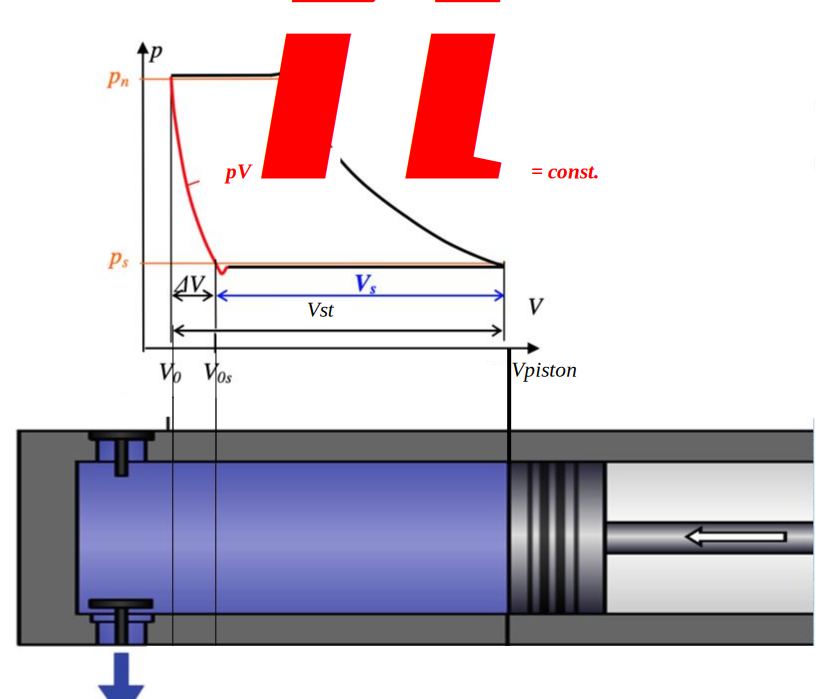
\includegraphics[width=0.4\textwidth]{figs/workcycle_real_v3.png}
\caption{\label{pistoncomp_pv2} $p-V$ diagram of the piston compressor's realistic working cycle. The red line is the polytropic expansion of the gas in the clearance volume $V_0$}
\end{center}
\end{figure}

The volumetric flow rate at the suction side can be calculated using the usual formula of positive displacement pumps:

\begin{equation} \label{eq_pistonvolflow1}
Q_s = \eta_v n V_s(p_s).
\end{equation}

Before gas enters the piston in the intake phase, first the gas in the clearance volume $V_0$ expands, until it reaches the suction side pressure. 
In Figure \ref{pistoncomp_pv2}, this expansion, which can be assumed to be a polytropic process, is displayed in red. The equation of the expansion is the following:

\begin{equation}
p\cdot V^n = \mathrm{const.} = p_p \cdot V_0^n =p_s V_{0,s}^n,
\end{equation}

in which $V_{0,s}$ is the volume at the end of the expansion. Rearranging yields

\begin{equation} \label{eq_clearanceexpansion}
V_{0,s} = V_0 \Big(\frac{p_p}{p_s}\Big)^{1/n}.
\end{equation}

%\begin{multline}
%V_s = V_{st} - \Delta V = V_{st} - (V_{0,s} - V_0) = V_{st} - \Bigg( V_0 \Big( \frac{p_p}{p_s} \Big)^{1/n} - V0 \Bigg) = \\
% V_{st} -  V_0 \Bigg( \Big( \frac{p_p}{p_s} \Big)^{1/n} - 1 \Bigg) = 
%\end{multline}

To calculate the volumetric flow rate, we would like to know the function $V_s(p_s)$. We find this using the geometric relation which can be read from Figure \ref{pistoncomp_pv2}:

\begin{equation}
V_s = V_{st} - \Delta V = V_{st} - (V_{0,s} - V_0) = V_{st} - \Bigg( V_0 \Big( \frac{p_p}{p_s} \Big)^{1/n} - V0 \Bigg) = V_{st} -  V_0 \Bigg( \Big( \frac{p_p}{p_s} \Big)^{1/n} - 1 \Bigg),
\end{equation}
where we also used Eq. \ref{eq_clearanceexpansion}. Finally, the formula is 

\begin{equation}
V_s = V_{st} \Bigg[1-\frac{V_0}{V_{st}} \Bigg( \Big(\frac{p_p}{p_s}\Big)^{1/n} - 1 \Bigg) \Bigg]
\end{equation}

Substituting this to Eq. \ref{eq_pistonvolflow1}, we get:

\begin{equation} \label{pistoncomp_Qs}
Q_s = \eta_v n V_{st} \frac{V_s}{V_{st}} = \eta_v n V_{st} \Bigg[1-\frac{V_0}{V_{st}} \Bigg( \Big(\frac{p_p}{p_s}\Big)^{1/n} - 1 \Bigg) \Bigg]
\end{equation}

To determine the pressure side volumetric flow rate, we can use the conservation of mass:
\begin{equation}
Q_s \rho_s = \dot{m} =  Q_p \rho_p.
\end{equation}

\begin{figure}[!h]
\begin{center}
\includegraphics[width=0.7\textwidth]{figs/workcycle_real.png}
\caption{\label{pistoncomp_pv2} $p-V$ diagram of the piston compressor's real working cycle.}
\end{center}
\end{figure}



\subsection{Control of flow rate}
\begin{description}
\item[Change revolution number] As it is obvious from Eq. \ref{pistoncomp_Qs}, $Q_s(s)$ is a linear function of $n$.

\item[Suction side valve / bypass] Similarly to pumps and fans, these control techniques can be utilized easily. 

\item[Adjustable clearance volume] The clearance volume $V_0$ affects the volumetric flow rate, which is obvious from Eq. \ref{pistoncomp_Qs}. By changing the clearance volume, the volumetric flow rate can be adjusted.

\item[Inlet valve unloaders] The suction side valve is not allowed to close fully, which means that during the compression process, a portion of the gas goes backwards in the suction pipe. 
\end{description}

\subsection{Multistage compressors}

It is often advantegous to split a compression cycle to two or more stages and use an intercooler between the stages.

\fbox{more text}

Consider the case of two stages, the first compressing from $p_s$ to $p_x$, while the second one from $p_x$ to $p_p$. We are searching for the intermediate pressure $p_x$ giving the lowest power, that is, the lowest specific work. The specifiy work of the two stages are (see \eqref{eq:chap1_polytropic_specific_work})
%
\begin{equation}
Y_{s\rightarrow x}=R T_s \frac{n}{n-1}\left( \left( \frac{p_x}{p_s}\right)^{\frac{n-1}{n}}-1 \right) 
\quad \text{and} \quad
Y_{x\rightarrow p}=R T_s \frac{n}{n-1}\left( \left( \frac{p_p}{p_x}\right)^{\frac{n-1}{n}}-1 \right).
\end{equation}
%
Note that due to the intercooler, the initial temperature of stage 2 is $T_s$ (instead of $T_p$). The optimal pressure will give $\sum Y(p_x)=Y_{1\rightarrow x}+Y_{x\rightarrow 2} \rightarrow \text{min}$, that is

\begin{align}
0&=\frac{d}{d p_x} \left( Y_{1\rightarrow x}+Y_{x\rightarrow 2}\right)\nonumber\\
0&=
\left(\frac{p_x}{p_s}\right)^{-\frac{1}{n}} \frac{1}{p_s}+
\left(\frac{p_p}{p_x}\right)^{-\frac{1}{n}} \left(-\frac{p_p}{p_x^2}\right)\nonumber\\
\left(\frac{p_x}{p_s}\right)^{-\frac{1}{n}} \frac{p_x}{p_s}&=
\left(\frac{p_p}{p_x}\right)^{-\frac{1}{n}} \left(-\frac{p_p}{p_x}\right)\nonumber\\
\frac{p_p}{p_x} &= \frac{p_x}{p_s}\nonumber\\
p_x&=\sqrt{p_s p_p}.
\end{align}

For example, for $p_s=1$ bar  and $p_p=8$bar, we have $p_x=2.83$ bar is the optimal interstage pressure. The specific work for the one-stage compressor would be ($R=287$kJ/kg, $T_s=293$K, $n=1.3$) 224 kJ/kg, where for the two-stage case, we have $Y_{1\rightarrow x}=Y_{x\rightarrow 2}=98.8$ kJ/kg (each), which gives $2\times98.8/224=88\%$ of the single-stage case.

\subsection{Problems}
%%%%%%%%%%%%%%%%%%%%%%%%%%%%%%%%%%%%%%%%%%%%%%%%%%%%%%%
% 13.1
\vspace{1cm}
\noindent {\bf Problem \thesection.\theprob}\stepcounter{prob}

We compress air ($R=287~\frac{\mathrm{J}}{\mathrm{kg\cdot K}}$) with temperature $t=20^\circ \mathrm{C}$ from $p_s=1~\mathrm{bar}$ to $p_n = 5~\mathrm{bar}$ using a piston compressor. The heat transfer between the air and the wall is not negligible (the compression is not adiabatic), and because of this the compression can be characterized with a polytropic coefficient $n=1.3$. The stroke volume is $V_{st} = 50~\mathrm{cm^3}$, the volumetric efficiency is $\eta_v = 98\%$, and the speed of the compressor is $n=740~\frac{1}{\mathrm{min}}$. The clearance volume is $6\%$ is the stroke volume. Find the
\begin{itemize}
\item suction side volumetric flow rate,
\item power of the compression, 
\item and the pressure side volumetric flow rate!
\end{itemize}

Solution:

The swept volume $V_s$ is 
\begin{equation}
V_s = V_{st} \Bigg[1-\frac{V_0}{V_{st}} \Bigg( \Big(\frac{p_p}{p_s}\Big)^{1/n} - 1 \Bigg) \Bigg] = 50\cdot \Bigg[1-0.06\cdot \Bigg( \Big(\frac{5}{1}\Big)^{1/1.3} - 1 \Bigg) \Bigg] = 42.65~\mathrm{cm^3}.
\end{equation}

From this, the volumetric flow rate at the suction side is
\begin{equation}
Q_s = \eta_v n V_s = 0.98\cdot 740 \cdot 0.04265 = 30.93~\frac{\mathrm{dm^3}}{\mathrm{min}} = 5.155\cdot 10^{-4}~\frac{\mathrm{m^3}}{\mathrm{s}}.
\end{equation}

The power is the following:
\begin{multline}
P_u = \dot{m} \oint \frac{\mathrm{d}p}{\rho(p)} = \dot{m} \frac{p_s^{1/n_{2-3}}}{\rho_s} \oint \frac{dp}{p_s^{1/n_{2-3}}} = \frac{\dot{m}}{\rho_s} p_s \frac{n}{n-1} \Bigg[ \Big(\frac{p_p}{p_s}^{\frac{n-1}{n}} -1 \Bigg] = \\
Q_s p_s \frac{n}{n-1} \Bigg[ \Big(\frac{p_p}{p_s}^{\frac{n-1}{n}} -1 \Bigg] = Q_s \cdot 10^5 \cdot \frac{1.3}{0.3} \Big[ 5^{\frac{0.3}{1.3}}-1\Big] = 194903\cdot Q_s
\end{multline}

During the compression the density of the gas increases, therefore the pressure side volumetric flow rate is lower than it is at the suction side:

\begin{equation}
Q_p = Q_s \frac{\rho_s}{\rho_p} = Q_s \Big(\frac{p_s}{p_p}\Big)^{1/n} = 30.93\cdot \Big( \frac{1}{5} \Big)^{1/1.3} = 8.968~\frac{\mathrm{dm^3}}{\mathrm{min}}
\end{equation}


The volumetric flow rate is $\dot{m} = Q_s \rho_s = 0.037~\frac{\mathrm{kg}}{\mathrm{min}}$. 

%%%%%%%%%%%%%%%%%%%%%%%%%%%%%%%%%%%%%%%%%%%%%%%%%%%%%%%
% 13.2
\vspace{1cm}
\noindent {\bf Problem \thesection.\theprob}
\setcounter{prob}{\value{prob}-1}

Using the data of problem {\bf \thesection.\theprob}, how does the suction side volumetric flow rate and the mass flow rate change, if we increase the clearance volume to be 40\% of the previous stroke volume!

\stepcounter{prob}\stepcounter{prob}

Approximating air as an ideal gas, we get

\begin{equation}
\rho_s = \frac{p_s}{RT_s} = \frac{100000}{287\cdot 293} = 1.189~\frac{\mathrm{kg}}{\mathrm{m^3}} = 0.001189~\frac{\mathrm{kg}}{\mathrm{dm^3}}
\end{equation}

The new clearance volume is $V_0' = 0.4\cdot V_{st}$, and substituting this to the formula of the swept volume yields

\begin{equation}
V_s' = V_{st} \Bigg[1-\frac{V_0'}{V_{st}} \Bigg( \Big(\frac{p_p}{p_s}\Big)^{1/n} - 1 \Bigg) \Bigg] = 50\cdot \Bigg[1-0.4\cdot \Bigg( \Big(\frac{5}{1}\Big)^{1/1.3} - 1 \Bigg) \Bigg] = 1.024~\mathrm{cm^3}.
\end{equation}

The new volumetric flow rate is

\begin{equation}
Q_s' = \eta_v n V_s' = 0.98\cdot 740 \cdot 0.001024 = 0.742~\frac{\mathrm{dm^3}}{\mathrm{min}},
\end{equation}

and using the suction side density, we can find the mass flow rate

\begin{equation}
\dot{m}' = \rho_s Q_s' = 0.001189\cdot 0.742 = 8.8\cdot 10^{-4}~\frac{\mathrm{kg}}{\mathrm{min}}.
\end{equation}

This is only 2.3\% of the original volumetric flow rate ($\dot{m} = 0.037~\frac{\mathrm{kg}}{\mathrm{min}}$), so the compressor is basically useless. It is important to note that changing the clearance volume is a widely used control technique.

%%%%%%%%%%%%%%%%%%%%%%%%%%%%%%%%%%%%%%%%%%%%%%%%%%%%%%%
% 13.3
\vspace{1cm}
\noindent {\bf Problem \thesection.\theprob}
\setcounter{prob}{\value{prob}-2}

Using the data of problem {\bf \thesection.\theprob}, find the power of the compression, if the compression is carried out in two steps, during which at the intermediate pressure $p=2.236~\mathrm{bar}$. Between the two compression steps, the air is cooled down such that the ration of the first and second piston volumes is $\frac{V_{piston,1}}{V_{piston,2}} = \frac{1}{2.236}$. For simplicity, assume that the clearance volume is in both cases $V_0 = 0$.!

(Solution: $P_u = 106.88~\mathrm{W}$)

\stepcounter{prob}\stepcounter{prob}\stepcounter{prob}
%%%%%%%%%%%%%%%%%%%%%%%%%%%%%%%%%%%%%%%%%%%%%%%%%%%%%%%
% 13.4
\vspace{1cm}
\noindent {\bf Problem \thesection.\theprob}\stepcounter{prob}

Find the number of stages in a piston compressor, which compressed nitrogen from $t_s = 20^\circ\mathrm{C}$ and pressure $p_s = 1~\mathrm{bar}$ to $p_n = 100~\mathrm{bar}$ absolute pressure! The criterion of the compression is that the temperature of the gas cannot exceed $t_{limit} = 140^\circ \mathrm{C}$! Because nitrogen gas molecules consist of two atoms, it is very similar to air, therefore the specific heat ratio can be assumed to be $\kappa = 1.4$. The compression can be characterized by a polytropic coefficient $n=1.33$.

(Solution: 4)


\clearpage